\section{Установка, настройка и тестирование интернет-радио на локальном сервере}

Следующим шагом после выбора программного обеспечения AzuraCast было изучать документации с официального сайта. Следуя официальному руководству, была установлена виртуальная машина Ubuntu for Windows и произведена установка AzuraCast на неё.

\begin{figure}[H]
  \centering
  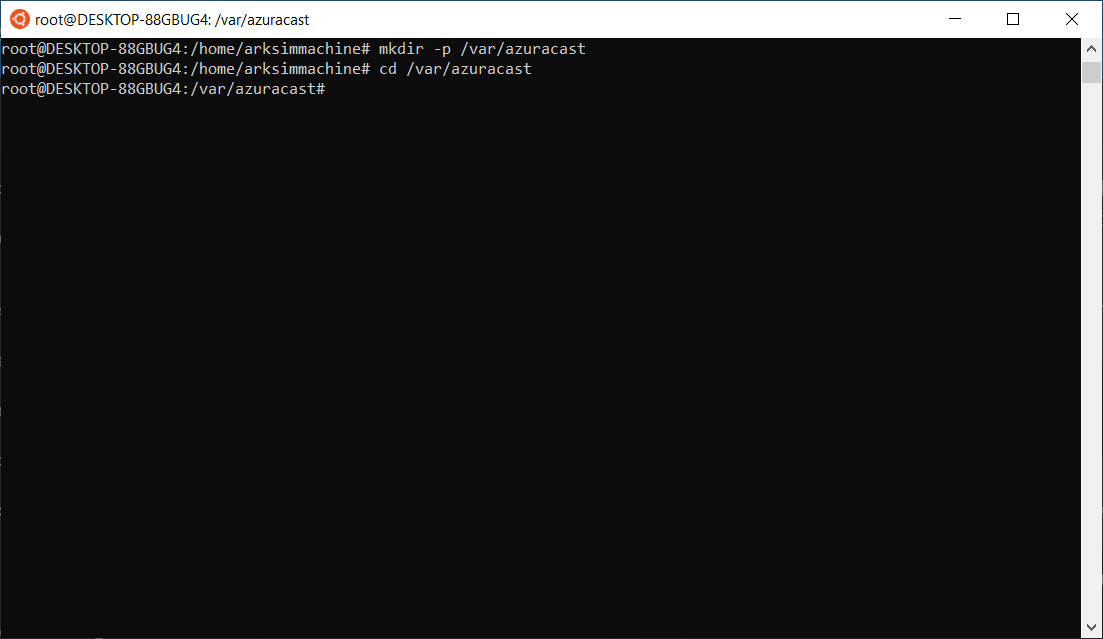
\includegraphics[interpolate, width=0.95\textwidth]{1}
  \caption{Установка AzuraCast на WSL}
  \label{fig:1}
\end{figure}

\begin{figure}[H]
  \centering
  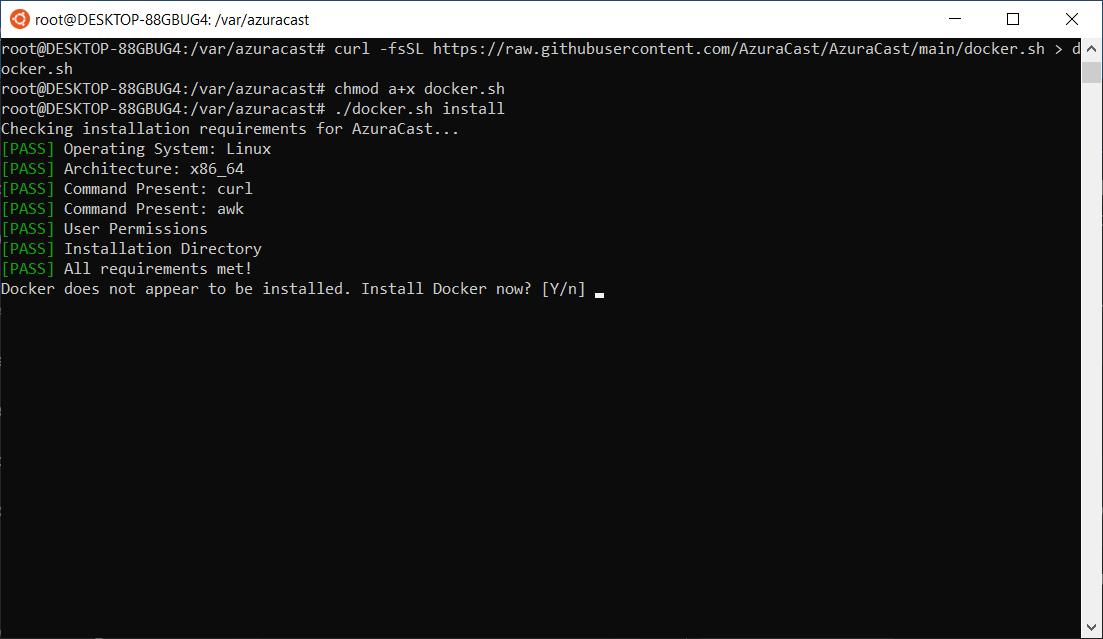
\includegraphics[interpolate, width=0.95\textwidth]{2}
  \caption{}
  \label{fig:2}
\end{figure}

\begin{figure}[H]
  \centering
  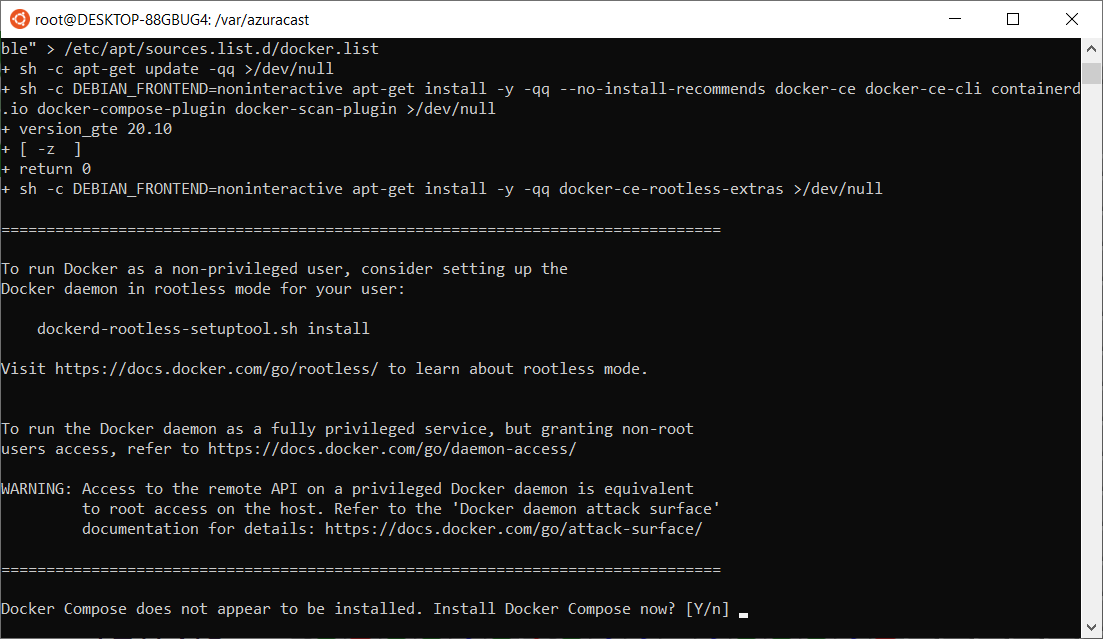
\includegraphics[interpolate, width=0.95\textwidth]{3}
  \caption{}
  \label{fig:3}
\end{figure}

\begin{figure}[H]
  \centering
  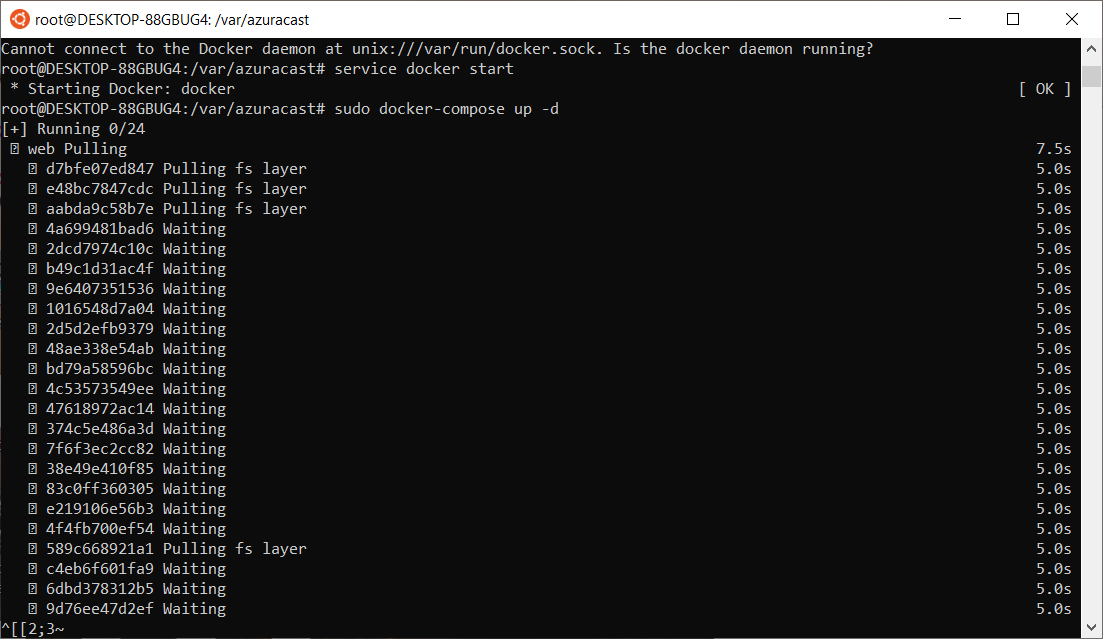
\includegraphics[interpolate, width=0.95\textwidth]{4}
  \caption{}
  \label{fig:4}
\end{figure}

\begin{figure}[H]
  \centering
  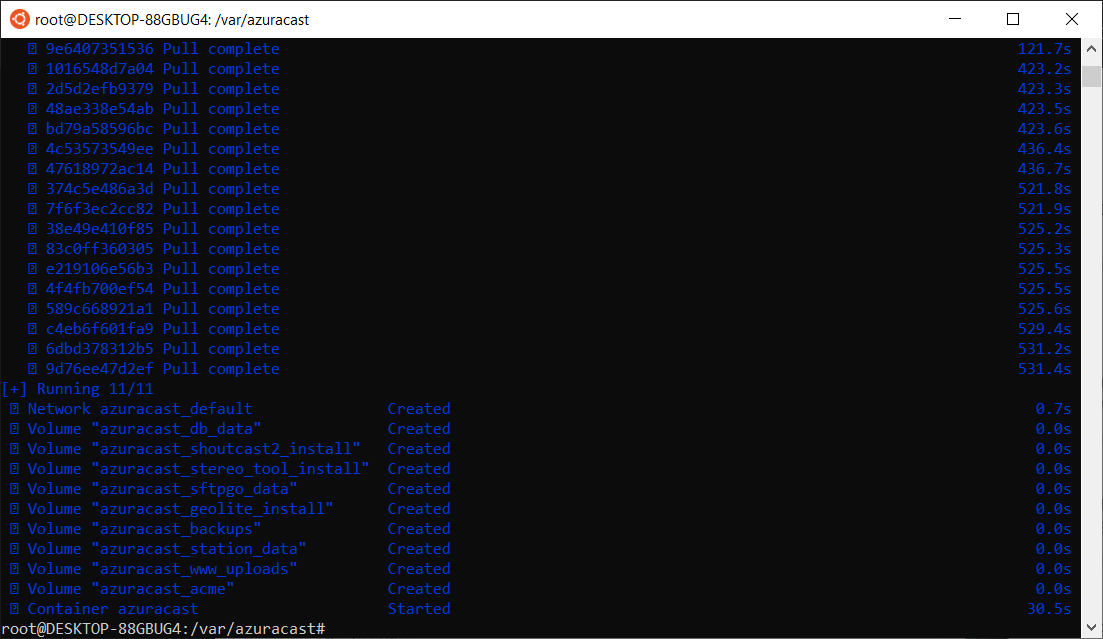
\includegraphics[interpolate, width=0.95\textwidth]{5}
  \caption{}
  \label{fig:5}
\end{figure}

После перехода по стандартному IP - 127.0.0.1, мы попадаем на окно первоначальной настройки.
\begin{figure}[H]
  \centering
  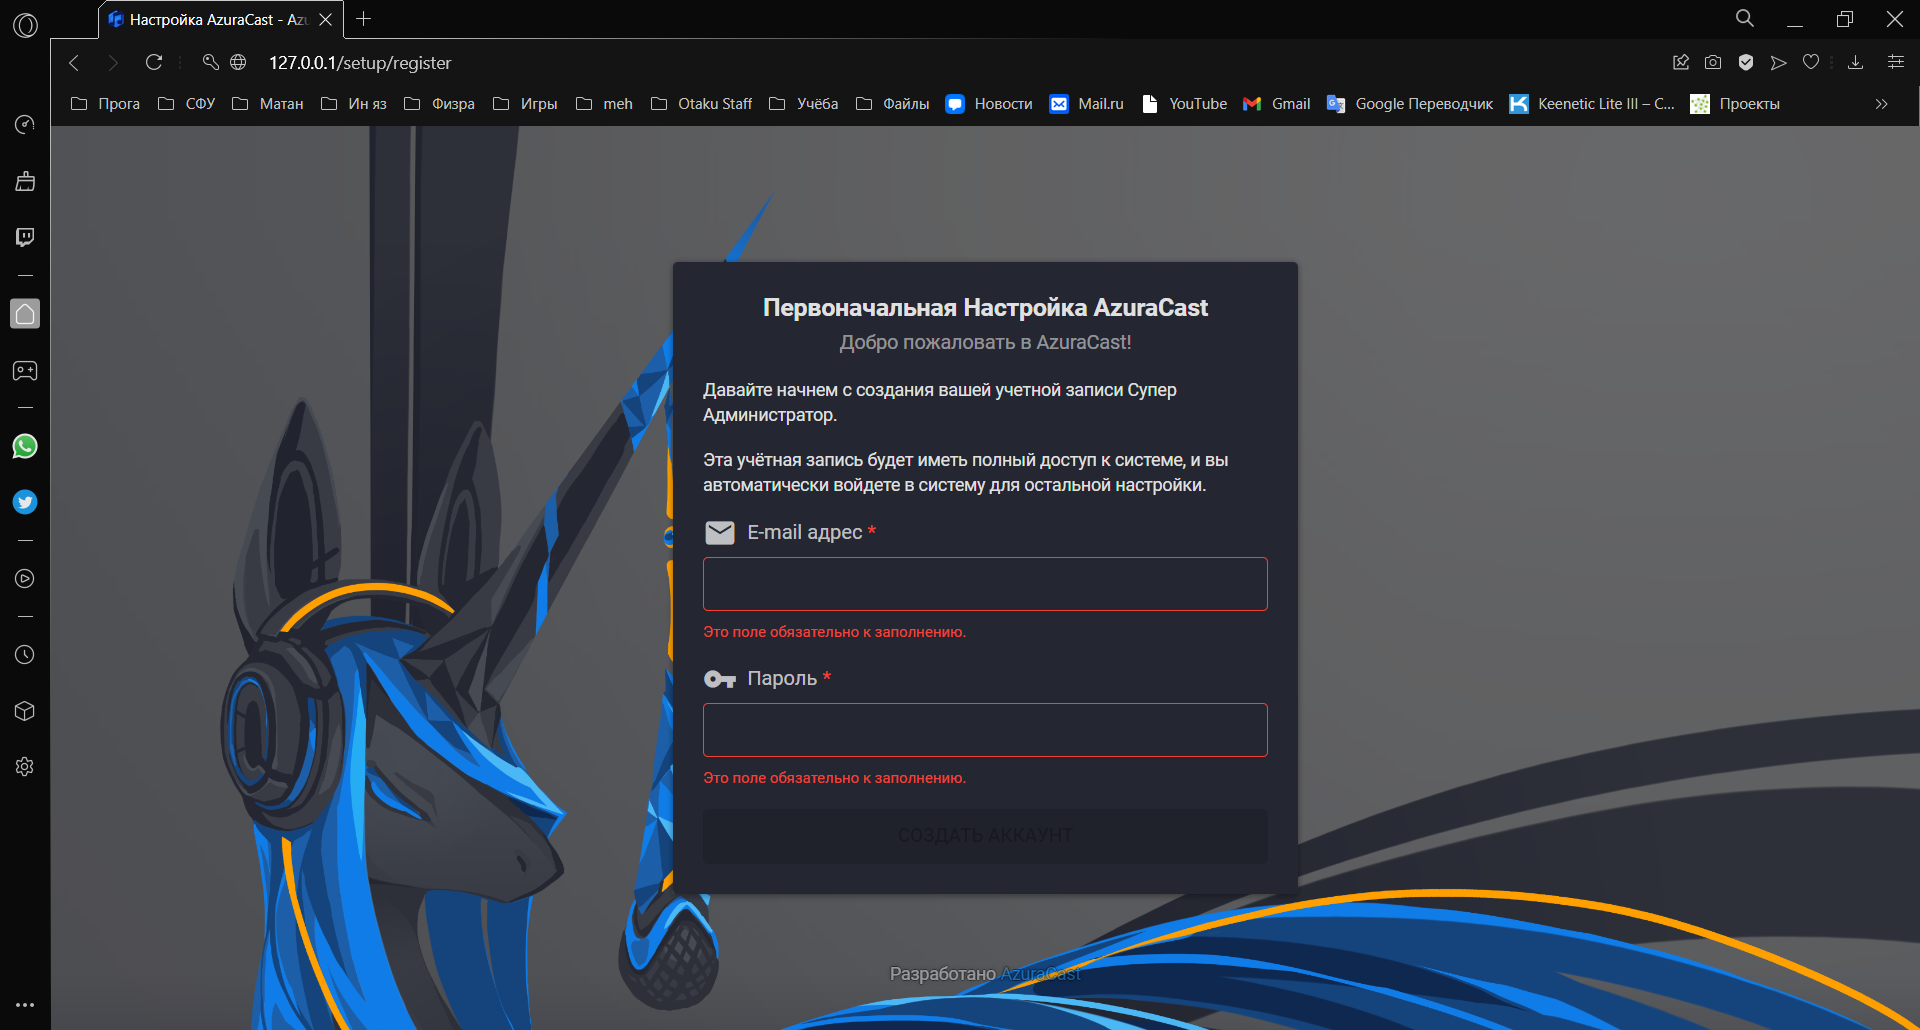
\includegraphics[interpolate, width=0.95\textwidth]{6}
  \caption{Окно настройки AzuraCast}
  \label{fig:6}
\end{figure}

Создаём пользователя.
\begin{figure}[H]
  \centering
  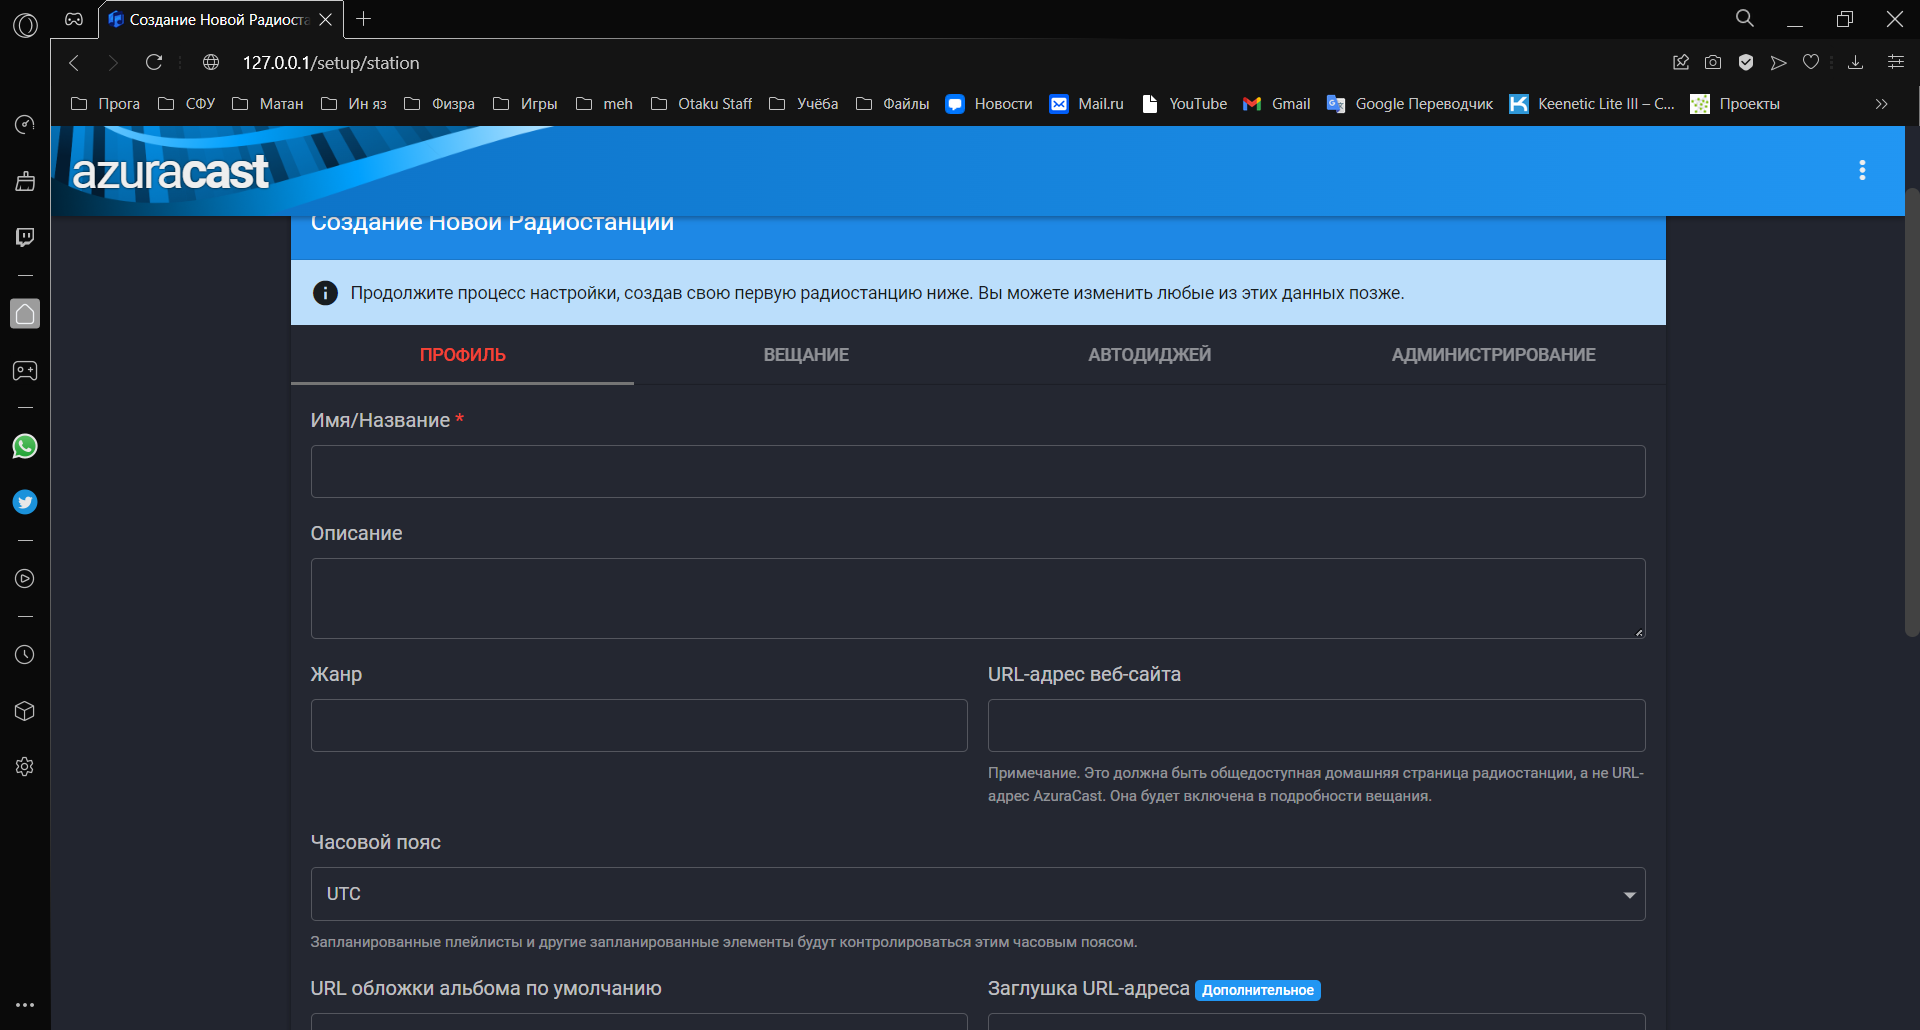
\includegraphics[interpolate, width=0.95\textwidth]{7}
  \caption{}
  \label{fig:7}
\end{figure}

Создаём радиостанцию.

Вписываем URL-адрес сайта.
\begin{figure}[H]
  \centering
  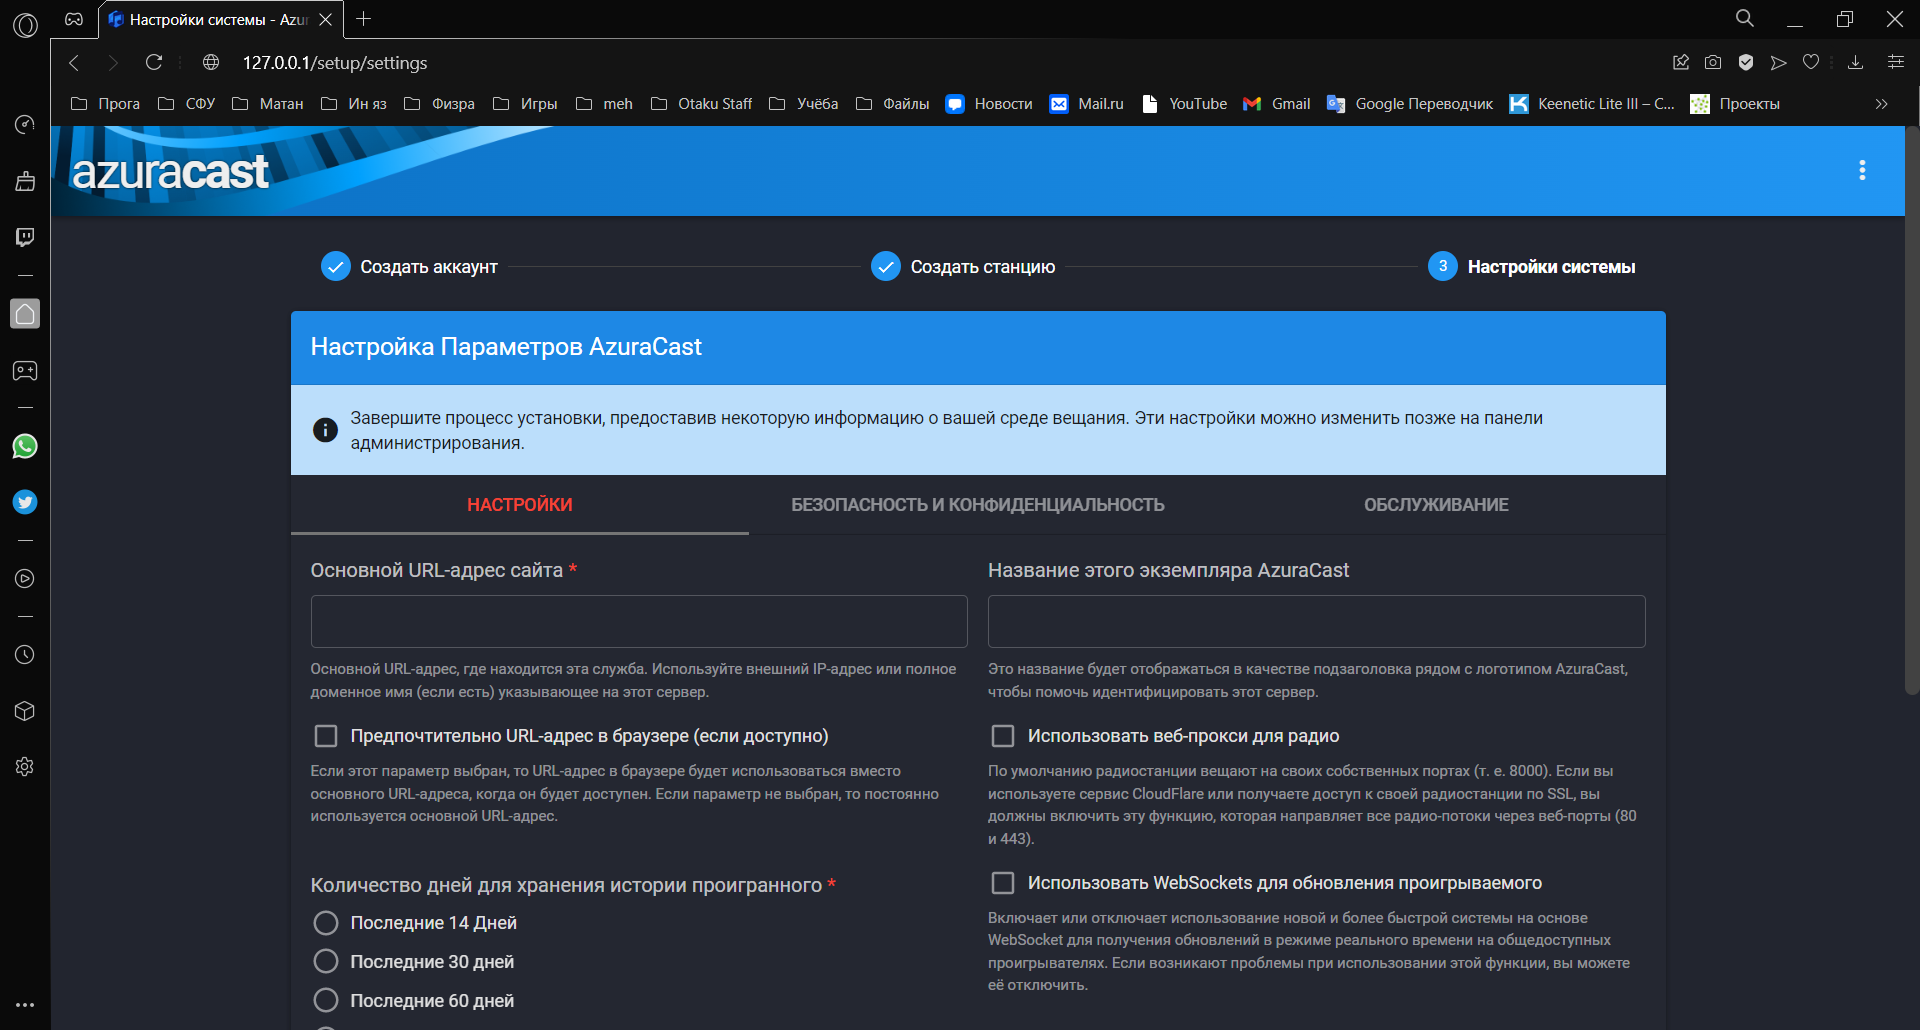
\includegraphics[interpolate, width=0.95\textwidth]{8}
  \caption{}
  \label{fig:8}
\end{figure}

После этого мы попадаем на окно управления самой радиостанцией. Дальше переходим в медиафайлы.
\begin{figure}[H]
  \centering
  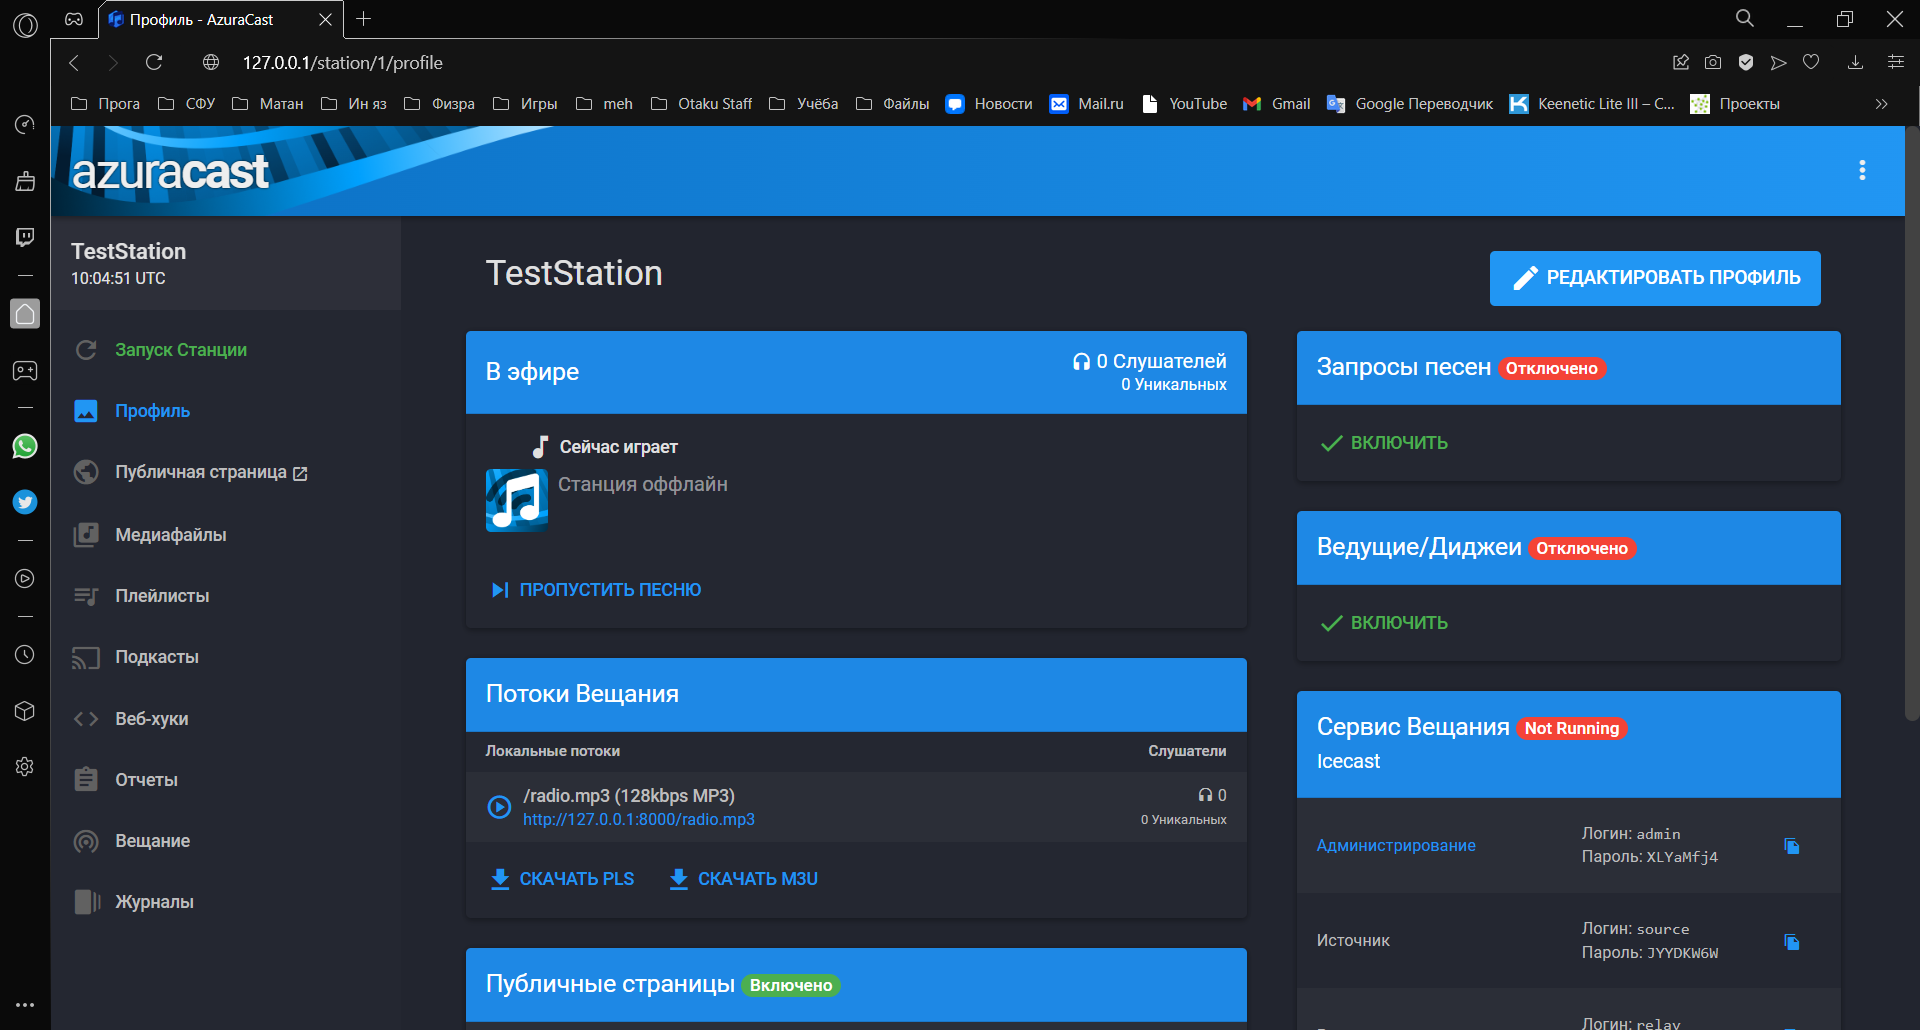
\includegraphics[interpolate, width=0.95\textwidth]{9}
  \caption{}
  \label{fig:9}
\end{figure}

Добавляем треки в хранилище сайта и добавляем их в плейлист default.
\begin{figure}[H]
  \centering
  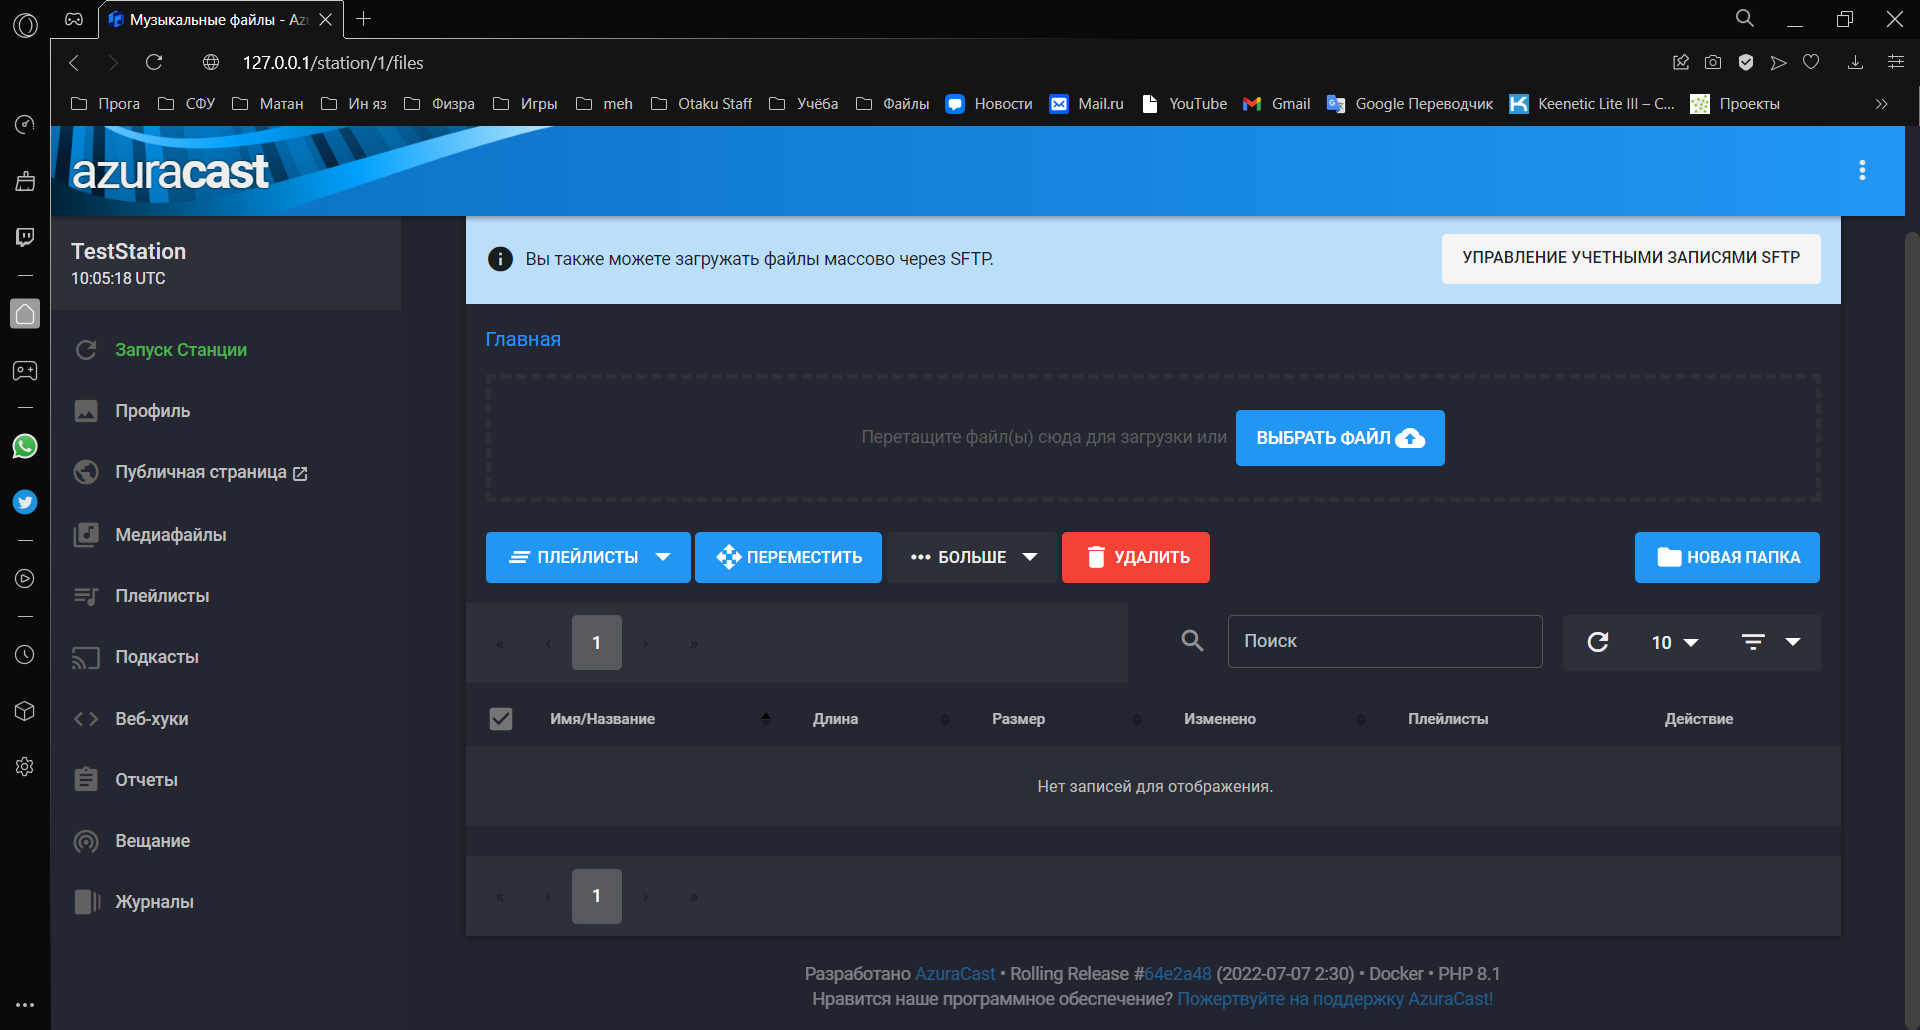
\includegraphics[interpolate, width=0.95\textwidth]{10}
  \caption{}
  \label{fig:10}
\end{figure}

После этого мы можем запустить станцию и перейти по адресу 127.0.0.1/public/teststation, чтобы протестировать работу.
\begin{figure}[H]
  \centering
  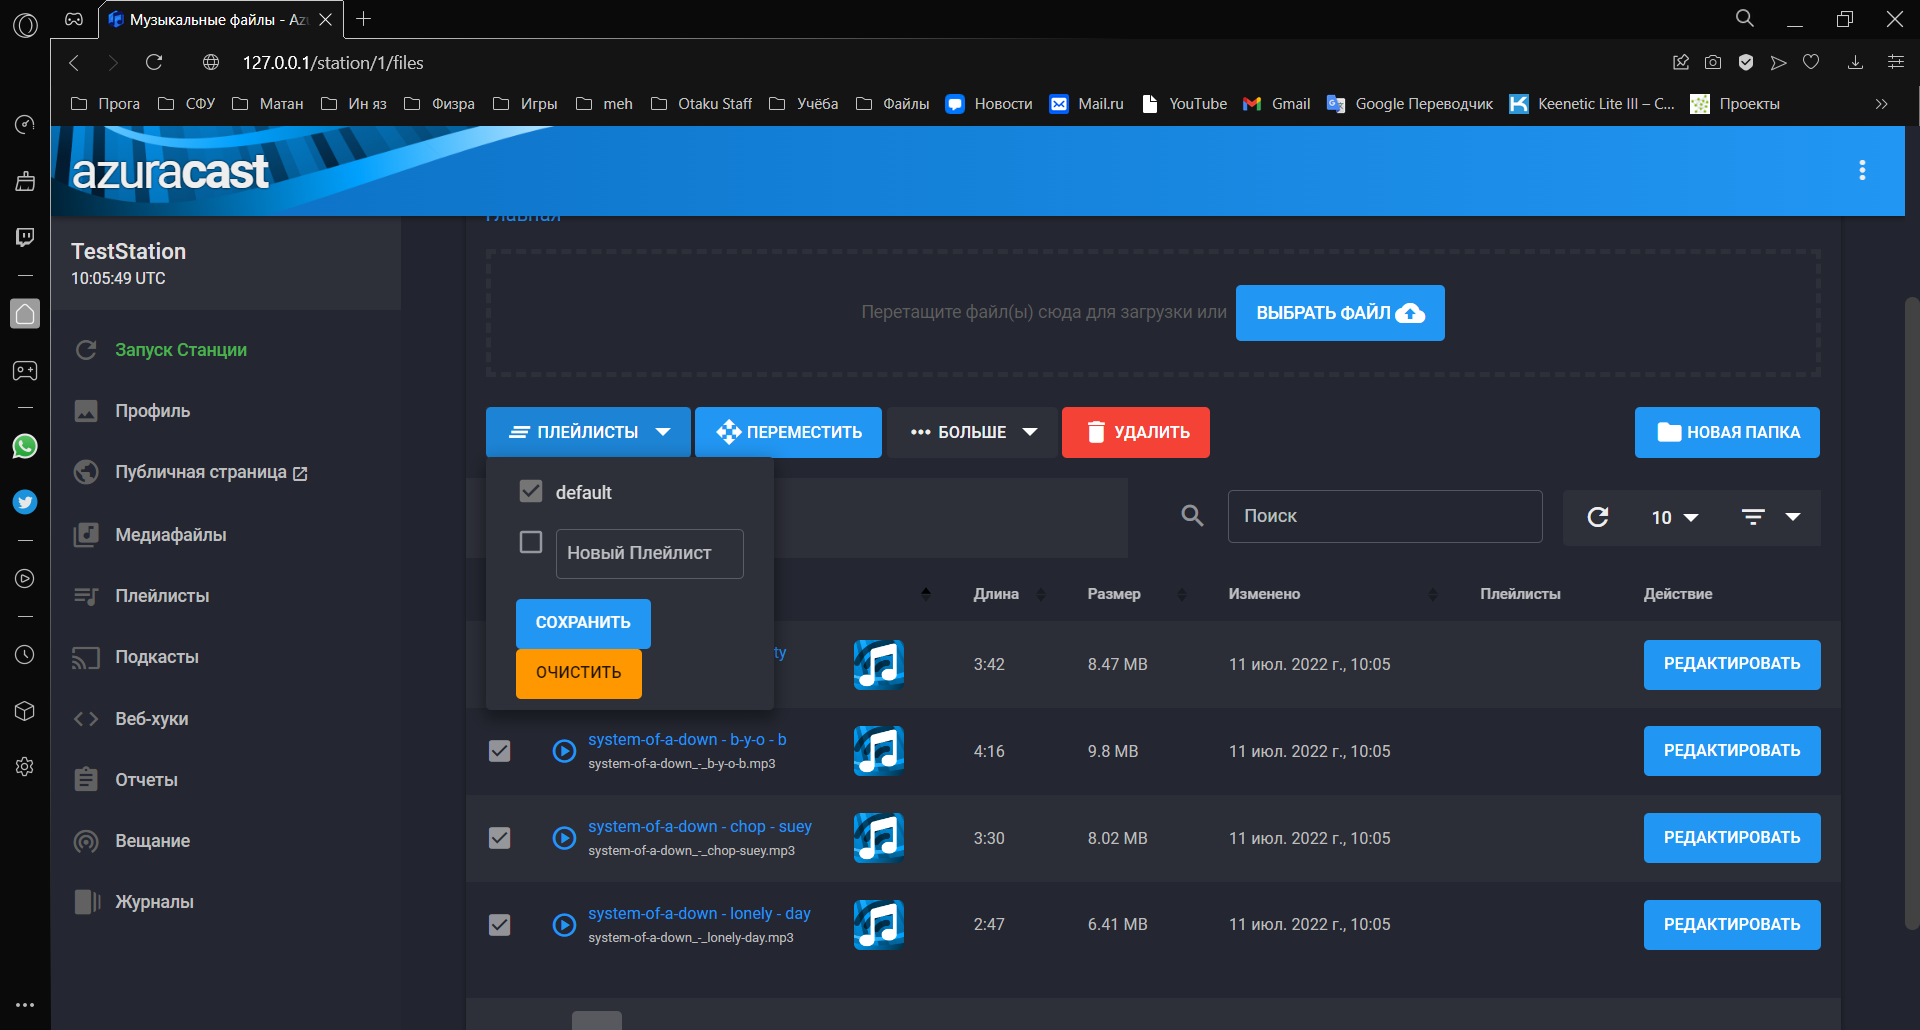
\includegraphics[interpolate, width=0.95\textwidth]{11}
  \caption{}
  \label{fig:11}
\end{figure}